\documentclass[11pt,a4paper,oneside]{article}
\usepackage[latin1]{inputenc}
\usepackage{amsmath}
\usepackage{amsfonts}
\usepackage{amssymb}
\usepackage{graphicx}
\usepackage{color}
\usepackage {tikz}
\usepackage{fancyvrb}
\usepackage{multicol}
\usepackage{caption}
\usepackage{subfig}
\usetikzlibrary {er}
\usepackage[left=2.00cm, right=2.00cm, top=1.00cm]{geometry}
\graphicspath{{./}}
\fvset{tabsize=4}

\begin{document}
	\title{DS 294 - Data Analysis and Visualization - Assignment 2}
	\author{Shriram R. \\ M Tech (CDS) \\ 06-02-01-10-51-18-1-15763}
	\maketitle	
	
	\section{Movelight}
	The \emph{movelight} example helps to demonstrate the utilities of lighting and transformation commands to render a model with a light which is moved by a modeling transformation. The following sections provide a description of interaction, functionalities of main \emph{OpenGL} functions and screenshots.

	\subsection{Interaction}
	The effects of interaction with the \emph{movelight} window is as follows,
	\begin{itemize}
		\item The light source is cyclically rotated around the 3D model in the horizontal plane by dragging the mouse pointer horizontally
		\item The position of camera or viewer is kept static irrespective of the light source position
		\item As the light source moves, part of the model is illuminated while the other part away from the source is shaded in black 
		\item The example provides a menu on right click which allows to select different models like Torus, Teapot, Dodecahedron, Tetrahedron, Icosahedron etc.
	\end{itemize}

   \subsection{Main OpenGL Functions}
   The following three are the primary OpenGL functions that were used in the example,
   \begin{itemize}
   	\item \textbf{\emph{glRotated}} - This function multiplies the current matrix by a rotation matrix. It takes angle, x, y and z coordinates as input and rotates the matrix. This function is used to rotate the light source by a specified angle when the mouse is dragged on the screen
   	\item \textbf{\emph{glTranslatef}} - This function multiplies the current matrix by a translation matrix. It takes x, y and z coordinates of the translation vector as input. This function is used to move the light source and model away from the camera and place them at a distance from the viewer
   	\item \textbf{\emph{gluPerspective}} - This function is used to setup a perspective projection matrix. It is takes field of view, aspect ratio, near and far clipping planes as input. This function is used to configure the world viewer properties and helps to capture the illuminated model
   \end{itemize}
   Other functions like \textbf{\emph{glLightfv}} to set position of light, \textbf{\emph{glutWireCube}} to draw a wire cube at the light etc. are also used in the example.
   
   \pagebreak
	
	\subsection{Screenshots}	
	The screenshots displayed in Figure~\ref{fig:movelight} are taken by interacting with the \emph{movelight} window.			
	\begin{figure}[!htbp]%
		\centering
		\subfloat[Torus with light source in front]{{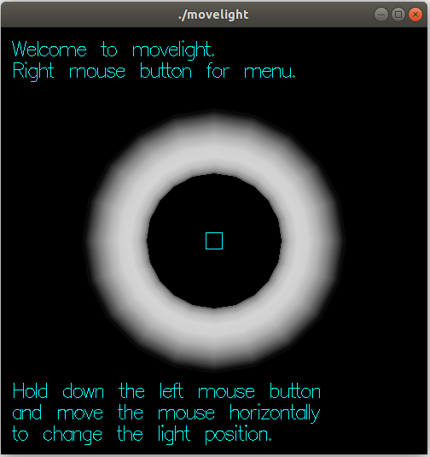
\includegraphics[width=7.5cm]{1.png} }}%
		\qquad
		\subfloat[Torus with light source in right]{{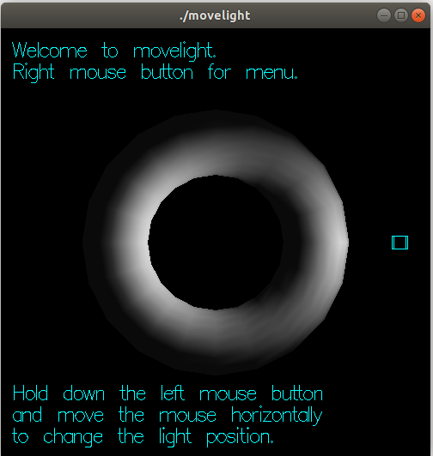
\includegraphics[width=7.5cm]{2.png} }}%
		\qquad
		\subfloat[Icosahedron with light source in front]{{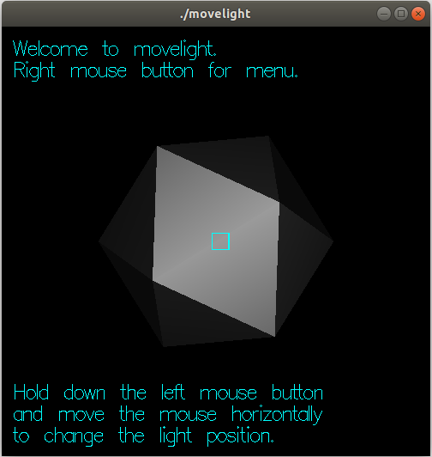
\includegraphics[width=7.5cm]{3.png} }}%
		\qquad
		\subfloat[Tetrahedron with light source in left]{{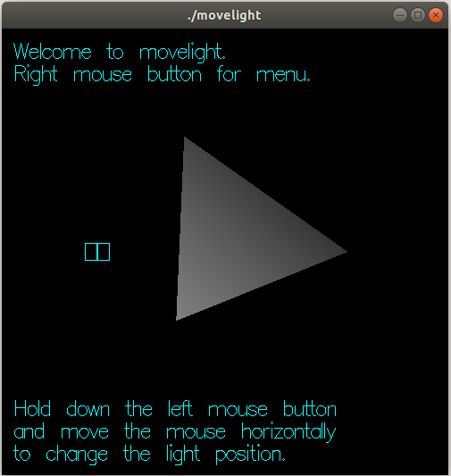
\includegraphics[width=7.5cm]{4.png} }}%
		\qquad
		\caption{Screenshots from \emph{movelight} example}
		\label{fig:movelight}%
	\end{figure}

%   \pagebreak
   
   \section{Multiple Windows}
   The \emph{multiple windows} example is used to demonstrate the functionalities of \emph{GLUT} which is the utilitiy module in displaying multiple windows at the same time. The following sections provide a description of interaction, functionalities of main \emph{OpenGL} functions and screenshots.
   
%   \pagebreak
   
   \subsection{Interaction}
   The effects of interaction with the \emph{multiple windows} window is as follows,
   \begin{itemize}
   	\item The program creates two separate windows which can moved and interacted independently of each other. The windows display a sphere with red and grey in color respectively
   	\item Each window comes with its own customized menu with different submenus and menu entries and can be accesses by right-click on the window. Clicking on the menu closes the window
   	\item The terminal running the program logs the status of mouse pointer when it enters/leaves the windows and keyboard presses with separate entries for each window 
   	\item The light source and camera is fixed in constant position in both the windows. The windows have different titles
   \end{itemize}
   
   \subsection{Main OpenGL Functions}
   The following three are the primary OpenGL functions that were used in the example,
    \begin{itemize}
   	\item \textbf{\emph{glutCreateMenu}} - This function is created a new pop-up menu. In this example, this function is used to create the custom menu for each window along with other function like \emph{glutAddSubMenu} to create submenus and \emph{glutAddMenuEntry} to create a new menu entry
   	\item \textbf{\emph{gluSphere}} - This function draws a sphere. It takes a quadric object, radius, slices (similar to lines of longitude) and stackes (similar to lines of latitude) as input. This function is used in the example to draw a sphere in each window
   	\item \textbf{\emph{gluLookAt}} - This function creates a viewing matrix from eye point, reference point (center of scene) and an up vector. It is used in the example to set the position and orientation of camera in the windows
   \end{itemize}
    Other \emph{GLUT} functions like \textbf{\emph{glutCreateWindow}}, \textbf{\emph{glutInitDisplayMode}} etc. are used in the example to create and set properties of the windows.
   
   \subsection{Screenshots}
   The screenshots displayed in Figures~\ref{fig:multiple1} \& \ref{fig:multiple2} are taken by interacting with \emph{multiple windows} example.
   	\begin{figure}[!htbp]%
   	\centering
   	\subfloat[Window 1 with red sphere]{{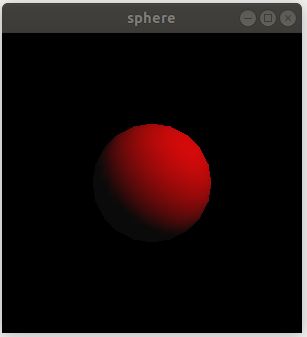
\includegraphics[width=7.5cm]{5.png} }}%
   	\qquad
   	\subfloat[Window 2 with grey sphere]{{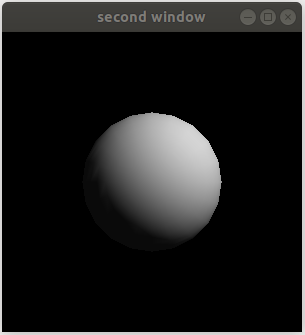
\includegraphics[width=7.5cm]{6.png} }}%
   	\qquad
   	\caption{Screenshots from \emph{multiple windows} example}
   	\label{fig:multiple1}%
   \end{figure}

   	\begin{figure}[!htbp]%
   	\centering
   	   	\subfloat[Mouse tracking log in console]{{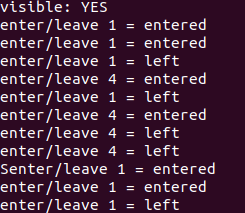
\includegraphics[width=7.5cm]{7.png} }}%
   	   	\qquad
   	   	\subfloat[Custom menu in the window]{{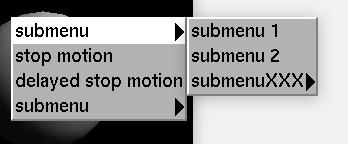
\includegraphics[width=7.5cm]{8.png} }}%
   	   	\qquad
   	\caption{Screenshots from \emph{multiple windows} example}
   	\label{fig:multiple2}%
   	\end{figure}
   
 
	
    \section{References}
    \begin{enumerate}
    	\item https://www.opengl.org/archives/resources/code/samples/glut\_examples/examples/examples.html
    	\item https://docs.microsoft.com/en-us/windows/desktop/opengl/glrotated
    	\item https://docs.microsoft.com/en-us/windows/desktop/opengl/gltranslatef
    	\item https://docs.microsoft.com/en-us/windows/desktop/opengl/gluperspective
    	\item https://www.opengl.org/resources/libraries/glut/spec3/node36.html	
    	\item https://docs.microsoft.com/en-us/windows/desktop/opengl/glusphere
    	\item https://docs.microsoft.com/en-us/windows/desktop/opengl/glulookat
    \end{enumerate}
 

    
\end{document}